% comment out one of the next two lines accordingly
% \documentclass[../thesis-main/main.tex]{subfiles}
\documentclass[../main.tex]{subfiles}
\usepackage{parskip}
\begin{document}

Please refer to Fig. \ref{fig:planning} for an overview of our planned work schedule.

% place figure here
\begin{figure}[h]
\centering
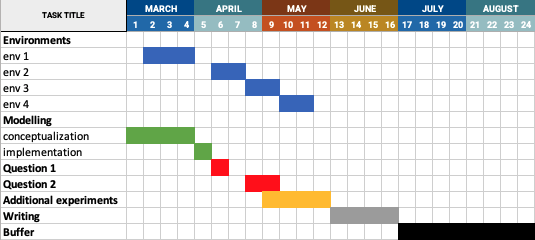
\includegraphics[width=\textwidth]{images/plan}
\caption{Overview of our planned work schedule. We intend to collect our results gradually, focusing
	one environment and one model at a time, starting from most simple and building from there.
	Because long term project planning is typically unrealistically optimistic, we plan for two months
	worth of ``buffer'' time at the end, which we will inevitably require. The plan is generally vague
	because the nature of research may cause large changes in direction that may render more detailed
planning obsolete.}
\label{fig:planning}
\end{figure}


\ifSubfilesClassLoaded{%
	\bibliographystyle{../../bibstyle}
	\bibliography{../../references-bibtex}%
}{}
\end{document}
